\cotefile{81}
\scanpage{49}
\unsure{$R$|$\mathcal{R}$} relation d'\unsure{équiva|équiv.} non \unsure{panachée|ponctuelle} sur $S$.

\uline{Segments} \inserted{$\underline{R}$} \uline{saturés} : \unsure{stable|stables} par passage au complémentaire, et par intersection et réunion quand celles-ci \deleted{\unsure{d}}donnent des segments (\inserted{p. ex. si} $A\cup B\ne S$, $A\cap B\ne\varnothing$)

Si $S_i\in\unsure{\mathcal{R}|R}$, alors les segments composants de $\complement S_i$ sont saturés, donc aussi leurs complémentaires i.e. les segments minimaux contenant $S_i$ (ou \inserted{segments} cocomposants de $S_i$). \deleted{Plus \unsure{général\textsuperscript{mt}|généralement}, si $T\subset S$ est une partie de $S$ $R$-saturée, alors les segments composants de}

\noindent\llap{\rule[-.92\baselineskip]{.4pt}{1.8\baselineskip}\hspace{.35em}}\uline{Prop} Les segments saturés minimaux sont les $\deleted{\unsure{A|S}}S_i\in R$ qui sont des segments.

% slanted
\reversemarginpar\margin{On appelle \unsure{les|ces} parties des \uline{onglets}}

Il est évident que si $S_i\in\deleted{\unsure{A}}R$ est un segment, alors c'est un segment saturé, et il est minimal parmi ces derniers (et $=$ parmi les parties saturées non vides). Inversement, soit $A$ segment saturé minimal, \deleted{\unsure{soit}} soit $S_i\in R$, $S_i\subset A$, \deleted{soit} je dis que $S_i=A$, \deleted{\unsure{ou|sin}} i.e. que l'on ne peut avoir $S_i,S_j\in R$ distincts, et
% slanted
\margin{\unsure{moitié|motif|mettant} du côté de la \unsure{section|notion|notation}}
\par\noindent\begin{minipage}[t]{.23\linewidth}
\vspace{0pt}
\figure{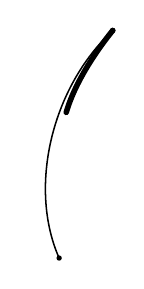
\begin{tikzpicture}[x=1cm,y=1cm,line cap=round,line join=round]
  \draw[line width=.55pt] (0.15,0) .. controls (-.24,.88) and (.04,2.15) .. (.83,2.89);
  \draw[line width=2pt] (.24,1.85) .. controls (.35,2.23) and (.62,2.63) .. (.83,2.89);
  \fill (.15,0) circle (.034) (.83,2.89) circle (.036);
\end{tikzpicture}}


\end{minipage}\hfill\begin{minipage}[t]{.73\linewidth}
\vspace{0pt}
$\subset A$. En effet, si $A_i$ $(A_j)$ est le \unsure{segm|segm.} cocomposant de $\deleted{\unsure{A}}S_i$ qui est contenu dans $A$, alors la condition que $S_i,S_j$ sont \deleted{\unsure{dis}}\unsure{non|bien} panachés s'exprime par la condition que $A_i\cap A_j=\varnothing$, donc $A_i,A_j$ sont des segments saturés $\subset A$ et $\ne A$, absurde.
\end{minipage}
\normalmarginpar
% archive sheet number: 48

